
\subsection{Model}

The Hubbard model\cite{Hubbard1963} describes spin-$\frac{1}{2}$ fermions with a density-density interaction:

\begin{equation}
\mathcal{H} = \sum_{i,j,\sigma} t_{ij} c^{\dagger}_{i,\sigma} c_{j,\sigma} + U \sum_{i} n_{i,\uparrow} n_{i,\downarrow}
\end{equation}

where $c^{\dagger}_{i,\sigma}$ and $c_{i,\sigma}$ are, respectively, creation and annihilation operators 
for fermions with spin $\sigma=\uparrow,\downarrow$. We consider the two-dimensional case with square lattice and repulsive interaction $U>0$ at finite temperature $T$ and in the SU(2) spin-symmetric phase. The hopping amplitude is restricted to $t_{ij} = t$ for nearest neighbors, $t_{ij}=t'$ for next-to-nearest neighbors. We take $t\equiv1$ as energy unit. 


\subsection{Flow equations}


In the following paragraph we will give some details about the functional renormalization group\cite{Metzner2012,Platt2013}, and we will clarify some notation issue about the vertex. 

Generally speaking, the fRG allows to use the renormalization group idea in the functional integral formalism. 
%This is done by endowing the non-interacting propagator $G_0$, and hence the action, with an additional dependence on a scale parameter $\Lambda$, which generates an exact functional flow equation\cite{Wetterich1993} with known initial conditions. The final result is recovered for some final $\Lambda$-value so that: $G_0^{\Lambda_\mathrm{f}} = G_0$. 

This is done by endowing the action with an additional dependence on a scale-parameter $\Lambda$:\cite{Metzner2012,Platt2013} 
\begin{equation}
 \mathcal{S}^\Lambda[\overline\psi,\psi]=
-(\overline\psi,{G_0^\Lambda}^{-1}\psi)+\mathcal{S}_{\mathrm{int}},  
\end{equation} 
where $\mathcal{S}_{\mathrm{int}}$ is the interaction part, and $(\overline\psi,\psi)$ summarizes the summation over all the quantum numbers of the fermionic fields  $\overline \psi$ and $\psi$. 
The scale dependence, acquired through the non-interacting propagator $G_0^\Lambda$, generates flow equations\cite{Wetterich1993} (with known initial conditions) for functional integrals, like the effective action, the effective interaction, or the generating functional for the connected Green's function. 
The final result is recovered for some final $\Lambda$-value so that: $G_0^{\Lambda_\mathrm{f}} = G_0$, and the original action is restored.  

We will apply this approach to the effective action, whose expansions into the fields generates the one-particle irreducible (1PI)  functions. By expanding the functional flow equation, one obtains a hierarchy of flow equations for the 1PI functions, involving vertices of arbitrarily  high orders. 
We will restrict ourselves to the two-particle level truncation by retaining only the two lowest nonvanishing orders in the expansion, i.e., we consider the flow of the self-energy $\Sigma^\Lambda$ and of the two-particle 1PI vertex $V^\Lambda$, neglecting the effects of higher order vertices. 
This truncation restricts the applicability of the approach to the weak-to-moderate coupling regime\cite{Salmhofer2001}. 
It can be furhter shown that, at the two-particle level trunctaion, the fRG sums up efficiently, although approximately, the so-called parquet-diagrams\cite{Binz2002,Binz2003,Kugler2017}. 

Due to translational invariance, we use the energy and momentum conservation to fix one of the arguments of the self-energy and of the vertex.  
Due to SU(2) symmetry, the self-energy is diagonal in spin-space: 
\begin{equation}
\Sigma^\Lambda_{\sigma\sigma'}(k)=\Sigma(k)\delta_{\sigma,\sigma'}, 
\end{equation}
where $k=(\nu,\mathbf{k})$, $\nu$ is a fermionic Matsubara frequency and $\mathbf{k}$ a momentum in the first Brillouin zone. 
\begin{figure}
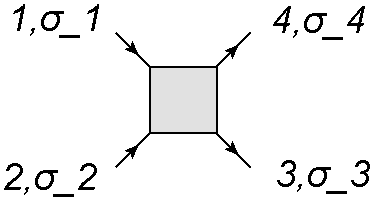
\includegraphics[width=0.15\textwidth]{images/VertexBox.png}
\caption{Notation of the two-particle vertex. \textbf{placeholder}
} 
\label{fig:notvert} 
\end{figure}

For the notation of the two-particle vertex function $V_{\sigma_1\sigma_2\sigma_3\sigma_4}(k_1,k_2,k_3)$ we refer to Fig.~\ref{fig:notvert}, where $k_i=(\nu_i,\mathbf{k_i})$.
% with $i\in\{1,2,3,4\}$,
 The momentum $k_4=k_1+k_2-k_3$ is fixed by conservation.%the other three and does not need to be specified.  
Furthermore  SU(2)-symmetry guarantees that the vertex does not vanish only for six spin combinations:
$
 V^\Lambda_{\uparrow\uparrow\uparrow\uparrow} = V^\Lambda_{\downarrow\downarrow\downarrow\downarrow}$, 
$  V^\Lambda_{\uparrow\downarrow\uparrow\downarrow} = V^\Lambda_{\downarrow\uparrow\downarrow\uparrow}  $, and
$  V^\Lambda_{\uparrow\downarrow\downarrow\uparrow } = V^\Lambda_{\downarrow\uparrow\uparrow\downarrow}$.   
Finally, due to SU(2) symmetry and crossing relation one has:\cite{Rohringer2012} 
\begin{eqnarray}
\nonumber
V^\Lambda_{\uparrow\uparrow\uparrow\uparrow}(k_1,k_2,k_3) &=& V^\Lambda_{\uparrow\downarrow\uparrow\downarrow}(k_1,k_2,k_3)\\&-& V^\Lambda_{\uparrow\downarrow\uparrow\downarrow}(k_1,k_2,k_1+k_2-k_3),
\label{eq:spinsym1}
 \\ 
V^\Lambda_{\uparrow\downarrow\downarrow\uparrow}(k_1,k_2,k_3)& =& -V^\Lambda_{\uparrow\downarrow\uparrow\downarrow}(k_1,k_2,k_1+k_2-k_3).
\label{eq:spinsym2}
\end{eqnarray}
This allows us to consider only one function of three arguments for the vertex:  $V^\Lambda(k_1,k_2,k_3)\equiv V^\Lambda_{\uparrow\downarrow\uparrow\downarrow}(k_1,k_2,k_3)$, all the others spin components being obtained by Eqns.~(\ref{eq:spinsym1}-\ref{eq:spinsym2}). 

With these considerations the flow equation for the self energy\cite{Metzner2012} reads: 
\begin{equation}
\frac{d}{d \Lambda} \Sigma^\Lambda(k)= -\int_p  S^\Lambda(p)\left[2V^\Lambda(k,p,p) -V^\Lambda(k,p,k)\right], 
\end{equation}
with $p=(\omega,\mathbf{p})$ and $k = (\nu,\mathbf{k})$. We use the notation  $\int_{p} =T\sum_\omega \int_{\mathbf{p}}$, $\int_{\mathbf{q}}=\int  \frac{d\mathbf{q}}{4\pi^2}$ being the normalized integral over the first Brillouin zone. 
\begin{equation}
 S^\Lambda=\frac{dG^\Lambda}{d\Lambda}\Bigg|_{\Sigma=\mathrm{const}} 
\end{equation}
  is the single-scale propagator and ${G^\Lambda}^{-1}=\left[(G_0^\Lambda)^{-1}-\Sigma^\Lambda\right]$ is the full propagator. 
  
 \begin{widetext} 
The vertex flow equation\cite{Metzner2012, Husemann2009} can be written as: 
\begin{align}
\label{eq:vertflow}
 \frac{d}{d\Lambda}V^\Lambda(k_1,k_2,k_3) =  \fl{\mathcal{T}}{pp}(k_1,k_2,k_3) +  
  \fl{\mathcal{T}}{ph}(k_1,k_2,k_3) + \fl{\mathcal{T}}{phc}(k_1,k_2,k_3),
\end{align} 
where:\footnote{The equation for the particle-particle channel is slightly different from the one usually reported in fRG, see, e.g., Ref. \onlinecite{Husemann2009}. This is because we took $\fl{V}{} = \fl{V}{\uparrow \downarrow \uparrow\downarrow}$ instead of $\fl{V}{} = \fl{V}{\uparrow\downarrow\downarrow\uparrow}$.  }
\begin{eqnarray}
\label{eq:ppT} 
\fl{\mathcal{T}}{pp}(k_1,k_2,k_3) &=&-\frac{1}{2} \int_p \fl{\mathcal{P}}{}(p,k_1+k_2-p) \Big\{  \fl{V}{}(k_1,k_2,k_1+k_2-p)\fl{V}{}(k_1+k_2-p,p,k_3) 
\label{eq:tpp} 
   \\ 
\nonumber
&&+  \fl{V}{}(k_1,k_2,p)\fl{V}{}(p,k_1+k_2-p,k_3) \Big\} ; \\  
\label{eq:tph} 
\fl{\mathcal{T} } {ph}(k_1,k_2,k_3) & =& -\int_p \fl{\mathcal{P}}{}(p,k_3-k_1+p)
\Big\{ 2 \fl{V}{}( k_1,k_3-k_1+p,k_3)  \fl{V}{}(p,k_2,k_3-k_1+p) \\
\nonumber
&&- \fl{V}{}( k_1,k_3-k_1+p,p)  \fl{V}{}(p,k_2,k_3-k_1+p) - \fl{V}{}( k_1,k_3-k_1+p,k_3)  \fl{V}{}(k_2,p,k_3-k_1+p) \Big\}; \\
\label{eq:tphc}
\fl{\mathcal{T}}{phc}(k_1,k_2,k_3) & =& \int_p \fl{\mathcal{P}}{}(p,k_2-k_3+p) \fl{V}{}(k_1,k_2-k_3+p,p)
\fl{V}{}(p,k_2,k_3).
\end{eqnarray} 
Here we have defined the quantity:
\begin{align}
\fl{ \mathcal{P }}{}(p,Q+p) &= G^\Lambda(p)S^\Lambda(Q+p) +G^\Lambda(p+Q)S^\Lambda(p),
\end{align} 
which is the scale-derivative, at fixed self energy, of a Green's function bubble with frequency and momentum transfer $Q$. 





